
\subsection{ Analiza kwestii bezpieczeństwa i przedstawienie znanych zagrożeń. }

\par
\tab W tej części zostaną przeanalizowane na dzień dzisiejszy znane podatności zarówno sieci opartych o protokół ZigBee jak i o Bluetooth Low Energy. Ponieważ obydwa rozwiązania jako swój fundament zakładają niski pobór energii przez podłączony węzeł, naturalną kwestią jest to, że obliczeniowo węzły nie są na dzień dzisiejszy implementować rozwiązań znanych z kryptografii asymetrycznej oraz bezpiecznych protokołów takich jak TLS czy SSL.\\
W zamian natomiast twórcy obu protokołów dołożyli największych starań aby oba te protokoły były jak najbardziej bezpieczne. \\

\par
\tab \textbf{ Bluetooth smart: \textit{"With low energy comes low security"}  }\\

Przeszukując sieć w poszukiwaniu narzędzi do ataku na Bluetooth Low Energy zetkniemy się napewno z najbardziej znanymi a mianowicie: projekt \textit{Ubertooth} oraz dobrze znany analizator pakietów sieciowych \textit{Wireshark} posiadający opcję analizy zarówno pakietów Bluetooth jak i również BLE.

	Na podstawie obecnych badań znanych jest kilka podatności sieci BLE, najbardziej znane to:
\begin{enumerate}
	\item Sniffing komunikacji
	\item Obchodzenie procesu parowania urządzenia
	\item Reużywanie tego samego klucza sesji	
\end{enumerate} 

\par
\tab \textbf{ "Sniffing Bluetooth Le is not hard" czyli o Sniffingu. }\\
-Powyższe hasło pochodzi z jednej z konferencji poświęconych bezpieczeństwu elektronicznemu, nawiązuje ono do hasła ktore stało się motywacją dla projektu Ubertooth[*]: "Sniffing Bluetooth is hard".\\
Jak zostało wcześniej wspomniane BLE jako protokół prowadzi transmisję na jednym z 37 kanałów transmisyjnych do wymiany danych, oraz korzysta z Techniki Hopping-u (po każdej wymianie pakietu zmienia kanał na numer obliczony poprzez dodanie wartości \textit{Hop Increment} do obecnego numeru) \\

\centerline{ $ NextChannel \equiv curren channel + hop increment (mod 37) $ } 
\mbox{}\\
Przykład komunikacji przy \textit{Hop Increment = 7} 
\mbox{}\\
\mbox{}\\
\centerline{ $ 3 \to 10 \to 17 \to 24 \to 31 \to 1 \to 8 \to 15 \to ... $ } 
\mbox{}\\
Algorytm Snifowania: 
	\begin{enumerate}
\item Ustaw częstotliwość odczytu na następny kanał
\item Następnie podąrzaj za transmisją uwzględniając hop inc
\end{enumerate} 
\mbox{}\\
\tab W celu przeprowadzenia takiego snifinu są wymagane jeszcze zmienne bezpośrednio związane z protokołem komunikacyjnym na którym posłuchujący chce odczytywać dane z kanału, a których to na początku nie zna: \textit{AccessAddress, CRCInit, Hop Interval, Hop Increment}. \\
Aby uzyskać AccessAddress należy skorzystać z faktu że w protokole wymieniane są puste pakiety które nie zawierają danych a służą jedynie do synchronizacji wymaganej przez hop internal. Taki pusty pakiet oprócz pustej liczby bitów posiada szukany adres. \\
CRCInit jest inicjalizującą sumą kontrolną na podstawie której obliczane jest CRC która służy do sprawdzania poprawność pakietu. Ponieważ liczenie CRC działa na podstawie rejestru przesuwającego z liniowym sprzężeniem zwrotnym da się je odzyskać odwracając tę liniową operację ["Bluesniff: Eve meets Alice and Bluetooth”, USENIX WOOT '07] \\
\tab HopInterval pozyskać można poprostu wyczekując na tym samym kanale 2 kolejnych pakietów z tym samym adresem. Ponieważ liczba 37 jest liczbą pierwszą mamy pewność, że niezależnie od kanału po pewnym czasie transmisja nastąpi na tym kanale.

\centerline{ $ \frac{\Delta t}{37 x 1.25 ms} = hop interval $ }
\mbox{}\\
Hop Increment można bardzo łatwo uzyskać po tym jak się otrzymało HopInterval, wystarczy poczekać na kanale 0 na transmisję a następnie wyczekiwać momentu w którym pojawi się pakiet na kanale 1-szym.
Ponieważ znamy HopInterval więc możemy policzyć jak dużo kanałów zostało przeskoczonych pomiędzy 0 i 1.
\mbox{}\\

\begin{gather*}
        0 + hopIncrement × channelsHopped  \equiv 1 (mod 37)\\
        hopIncrement \equiv  channelsHopped^{-1} (mod 37) \\
        channelsHoppped^{-1} \equiv channelsHopped^{37-2} (mod 37)
\end{gather*}

W efekcie czego otrzymujemy wszsytkie parametry połączenia które możemy zawsze w przyszłości śledzić ponieważ BLE domyślnie zapamiętuje parametry transmisji z urządzeniem aby w kolejnych komunikacjach nie marnować energii na ustalanie ich od początku. \\

\par
\tab \textbf{Obchodzenie mechanizmu parowania} \\
Jak wcześniej zostało wspomniane Bluetooth Low Energy w standardzie obsługuje mechanizm symetrycznego szyfrowania w oparciu o Algorytm szyfrujący AES - 128bitowy. Szyfrowanie odbywa się na warstwię łączącej (Link Layer) protokołu. Podczas procesu następuje szyfrowanie części pakietu PDU (Dla zobrazowania tego faktu poniżej została zaznaczona omawiana część pakietu na czerwono), natomiast pozostała część jest przesyłana w postaci jawnej.\\

\centerline{
	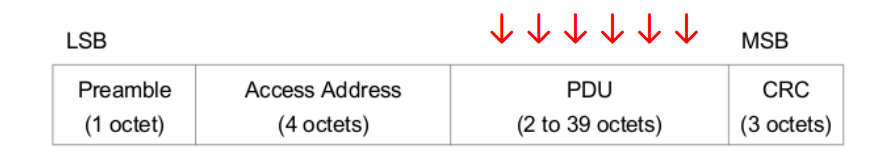
\includegraphics[scale=0.35]{./img/AES_PDU_crypt.png}
}
Trzy metody parowania urządzeń BLE
\begin{enumerate}
	\item Parowanie bez PIN-u
	\item 6 cyfrowy PIN
	\item PIN 00B	
\end{enumerate} 

\tab W celu przeprowadzenia szyfrowanej transmisji musi najpierw zostać wykonany proces wymiany klucza, nazywany potocznie parowaniem. Proces ten jest trójstopniowy, i podczas niego na początku obie strony uzgadniają między sobą TK (temporary key) poprzez 3 etapową wymianę danych za pomocą 3 parametrów: rand (liczba pseudolosowa), p1/p2 (parametry zależne od pinu, dla 00B są to zera). Parametry te są przesyłane między stronami \textbf{postaci jawnej w powietrzu}, za pomocą tych wartości obie strony wyliczają tzw \textit{confirm value}, po wyliczeniu którego komunikacja między stronami zaczyna być szyfrowana za pomocą TK, a następnie jest w ramach sesji STK (Short term Key) który służy do ustawienia bezpiecznego połączenia w ramach którego może być przesłany LTK (Long Term Key) którego w przyszłości strony będą używać do komunikacji.
Jednakże posiadająć TK, można odszyfrować STK oraz sesję a w efekcie czego LTK

Sposób rozszyfrowywania TK
\begin{gather*}
        configm = AES(TK, AES(TK, rand XOR p1) XOR p2)\\
        confirm, rand, p1/p2 są przesyłąne w postaci jawnej \\
        TK jest wartością od 0 do 999,999 dla PIN6 lub 0 dla JustWorks
\end{gather*}


\par
\tab \textbf{Reużywanie tego samego klucza sesji} \\

\tab Po tym opisie łatwo wywnioskować, że żadna z powyższych metod parowania nie zapewnia ochrony przeciwko pasywnemu podsłuchiwaniu. \\
Mało tego ponieważ protokół bluetooth LE był projektowany dla urządzeń wbudowanych zasilanych bateryjnie protokół uwzględnia mechanizm \textit{Counter-mitigation} który ma na celu zapewnienia możliwości ponownego uzgodnienia klucza w przypadku gdyby któreś z urządzeń straciło pamięć w wyniku rozładowania baterii. Skutkuje to możliwością podsłuchującego do wymuszenia celowej renegocjacji klucza, nawet gdy oba urządzenia zostały już poprawnie sparowane w bezpiecznym miejscu.
Atakujący który raz podsłucha procesu parowania jest w stanie odtworzyć TK, STK oraz LTK. 
Samo ustalenie TK za pomocą metod typu bruteforce zajmuje mniej niż 1 sekunde na 1 rdzeniu procesora intel i7 który nie ma sprzętowego wsparcia dla algorytmu AES, i umożliwiają to powszechnie dostępne w sieci narzędzia OpenSource. \\


\par
\tab \textbf{ ZigBee: \textit{and KillerBee}  }\\

Podobnie jak w przypadku poprzedniej części zostaną wymienione znane techniki ataków na sieci ZigBee, łącznie z omówieniem zasad ich działania.
Materiałów dotyczących samych podatności sieci ZigBee jest dużo mniej niż w przypadku innych protokołów bezprzewodowych ponieważ sam standard nie jest na tyle popularny w życiu codziennym jak ma to miejsce przy np 802.11 (Wifi) czy Bluetooth i BLE. Z otwartych narzędzi służących exploitacji oraz sniffingu protokołu ZigBee warto wymienić framework KillerBee czy narzędzie WireShark posiadające opcję sniffingu i analizy pakietów ZigBee.
Specyfikacja ZigBee zawiera w sobie szereg elementów przewidzianych do tego aby chronić \textit{"Poufności oraz integralności danych"}, głównymi z nich jest używanie standardu kryptograficznego AES oraz Autentykacji danych za pomocą klucza sieciowego. Dodatkowo standard ten definiuje dwa tryby bezpieczeństwa:
\begin{enumerate}
	\item \textbf{Standardowy tryb bezpieczeństwa} \textit{(Standard security mode)}: w którym to autentykacja każdego węzła odbywa się za pomocą współdzielonego klucza sieciowego dostarczanego i uwierzytelnianego przez Trust Center oraz Listy dostępu \textit{ACL (Access Control List)}
	\item \textbf{Tryb wysokiego bezpieczeństwa} \textit{High security mode} w tym trybie autentykacja jest dużo bardziej restrykcyjna ponieważ Trust Center trzyma wszystkie klucze szyfrujące oraz autentykujące używane w sieci. Z tego powodu musi dysponować one dodatkowymi zasobami aby być w stanie śledzić wszystkie urządzenia w sieci oraz odmawiać niechcianym urządzenią dostępu do sieci.	
\end{enumerate} 

Na podstawie obecnych badań oraz materiałów znane są następujące ataki na sieć ZigBee:
\begin{enumerate}
	\item Odkrywanie fizycznego połorzenia węzłów
	\item Sniffing pakietów
	\item Wstrzykiwanie pakietów
	\item Przechwytywanie transportu klucza (Tylko sieci w trybie Standardego trybu bezpieczeństwa)
\end{enumerate} 


\par
\tab \textbf{Odkrywanie fizycznego połorzenia węzłów} \\
Wszystkie układy radiowe które są emiterami emitują pole elektromagnetyczne. W przypadku standardu 802.15.4 układ radiowy może jako część protokołu zeskanować sieć i dla każdego odnalezionego adresu w sieci wyznaczyć jego siłę sygnału. Takie rozwiązanie jest bardzo pomocne przy tworzeniu sieci, debugowaniu czy diagnostyce, jednakże umożliwia ono również każdemu wyposażonemu w układ radiowy intruzowi na fizyczną lokalizację wszystkich urządzeń podłączonych do sieci. pakiet \textit{zbfind} wchodzący w skład frameworku KillerBee umożliwia prostą lokalizację urządzeń nadających w sieci fizycznej 802.15.4.
Atak polegający na znajdowaniu samych urządzeń warty wspomnienia ponieważ sieci ZigBee są stworzone do zastosowań przemysłowych w których najczęściej takie urządzenia są pozostawione "same sobie", przypominając sobie jakie urządzenie w sieci ZigBee decyduje o bezpieczeństwie całej sieci (Trust Center) widoczne jest że w prosty sposób napastnik może wyłączyć całą sieć. Dodatkowo należy wspomnieć o urządzeniach takich jak GoodFet które to implementuje interfejs JTAG (Join Test Action Group) służący do debugowania układów elektronicznych umożliwiający np. zrzut całej pamięci urządzenia w postaci binarnej mapy pamięci.
 \centerline{
	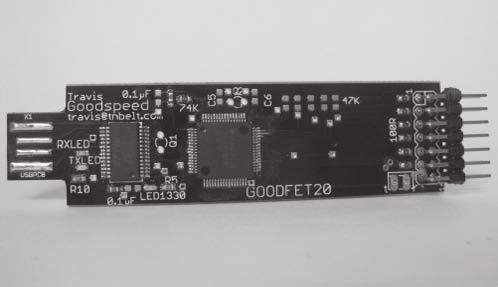
\includegraphics[scale=0.35]{./img/goodFet.jpeg}
}
Atak taki mógłby przebiegać w następujący sposób:
\begin{enumerate}
	\item Atakujący odkrywa fizyczne położenie węzłów sieci
	\item Atakujący znajduje Trust Center
	\item Za pomocą GoodFET Napastnik zyskuje dostęp do wszystkich kluczy sieciowych
\end{enumerate} 
Ponieważ dla pewnej rodziny popularnych chipów np firmy \textit{Texas Instruments} klucze są przetrzymywane w urządzeniu w postaci nie zaszyfrowanej, oraz w miejscu w pamięci dobrze opisanym w dokumentacji technicznej, ataku tego może dokonać prawie każdy wyposarzony w framework KillerBee oraz narzędzie GoodFET. \\

\par
\tab \textbf{Sniffing pakietów} \\
Ponieważ duża część dostępnych nadajników ZigBee nie wspiera domyślnie (lub czasem całkowicie) szyfrowanego połączenia, Atakujący może z łatwością w takich sieciach przechwycić cały ruch sieciowy. Szyfrowanie w sieciach ZigBee maskuje treść danych natomiast nie ukrywa MAC adresu oraz PAN ID, ten fakt w połączeniu z możliwością fizycznej lokalizacji odbiorników dostarcza dodatkowych możliwości ataku na sieć.\\
W przypadku sieci pracujących w trybie SSM (Standard Security Mode), w momencie przyłączenia nowego węzła do sieci po autentykacji, klucz sieciowy jest wysyłany do urządzenia w postaci nie zaszyfrowanej, a następnie za jego pomocą jest wymieniany \textit{Link Key} (LK jest wysyłany w postaci zaszyfrowanej za pomocą Network Key).\\ 
Powyższy scenariusz umożliwia podsłuchującemu napastnikowi który dołączy do sieci na przechwytywanie kluczy do innych nowych węzłów. Co więcej w momencie kiedy tworzona jest cała sieć a napastnik podsłuchuje komunikację jest w stanie poznać Network Key bez konieczności dołączania do sieci, wystarczy że podsłucha pierwszą wymianę klucza sieciowego, aby tego dokonać Atakujący może namierzyć fizycznie Koordynatora oraz kanał częstotliwości na którym działa sieć po czym po prostu zresetować zasilanie Koordynatora w efekcie czego sieć będzie tworzona od nowa, a napastnik podsłucha wymiany wszystkich kluczy. \\
Problem pasywnego podsłuchiwania rozwiązuje tryb HSM (High security mode) w którym to żadne klucze nie są wymieniane w postaci jawnej a zamiast tego są fabrycznie zapisywane w pamięci urządzeń. To rozwiązanie ma swoje wady jeśli chodzi o elastyczność takiego rozwiązania (np w razie ewentualnej awarii któregoś z urządzeń) ale w zamian za to dostarcza bezpieczne rozwiązanie komunikacyjne. \\

\par
\tab \textbf{Wstrzykiwanie pakietów} \\
Koncept ataku jest bardzo prosty: obserwacja pakietów oraz retransmisja wybranych pakietów (w przypadku sieci zaszyfrowanych) lub w przypadku znajomości kluczy albo sieci jawnych proste tworzewnie własnych pakietów. \\
Sam standard ZigBee zakłada niepodatność protokołu na ataki typu \textit{Reply Attacks} jednakże Autor do tej pory nie spotkał się z implementacją stosu ZigBee który by był odporny na te ataki. Np. dostawca dużego procenta chipów do ZigBee \textit{Texas Instrument} dostarcza stos do swoich układów który jest podatny na atak wstrzykiwania tego samego pakietu. \\
Wyobraźmy sobie taki scenariusz ataku:
\begin{enumerate}
	\item Napastnik poprzez znajomość fizycznego położenia węzłów sieci identyfikuje je z MAC adresami
	\item Atakujący podsłuchuje sieć i wywołuje pewne zdarzenia np. stymuluje sensory lub korzysta z dostępnych włączników/przełączników.
	\item Przy dużej próbie jest w stanie powiązać poszczególne pakiety ze zdarzeniami fizycznymi czy impulsami.
	\item Posiadając mapowanie pakiet-zdarzenie Napastnik może sterować siecią i wywoływać zdarzenia które podsłuchał. Dotyczy to zarówno szyfrowanych sieci (HSM, SSM) jak i jawnych.
\end{enumerate}  

\par
\tab \textbf{Przechwytywanie transportu klucza} \\
Standard ZigBee wprowadza dodatkowe mechanizmy służące rozprowadzaniu kluczy, takie jak prekonfiguracja (ustawienie klucza na urządzeniu podczas procesu wytwarzania) negocjacja klucza (Protokół \textit{SKKE - Symmetric-Key Key Establishment}). Prekonfiguracja jest wymagana w trybie \textit{HSM} zapewnia ono wysokie bezpieczeństwo ale również bardzo trudną późniejszą rekonfiguracje każdego z urządzeń w sieci.\\
Natomiast mechanizm SKKE wprowadzony w versji ZigBee-Pro umożliwia prostą i elastyczną rekonfigurację w oparciu o Trust Center. Niestety SKKE jest niewystarczającym mechanizmem zabezpieczającym i może być łatwo złamany albo podsłuchany tak jak to zostało wspomniane wcześniej. Z tego powodu we wszystkich zastosowaniach w których wymagane jest wysokie bezpieczeństwo należy wystrzegać się mechanizmów opartych o kryptografię symetryczną takich jak SKKE ponieważ w nich najczęściej występuje dystrybucja kluczy lub części klucza umożliwiająca atakującemu na złamanie klucza sesji (lub jego podsłuchanie).


